% !TEX encoding = UTF-8 Unicode
% !TEX TS-program = xelatex
% !BIB program = biber

% MIT License
%
% Copyright (c) 2019 Star Brilliant
%
% Permission is hereby granted, free of charge, to any person obtaining a copy
% of this software and associated documentation files (the "Software"), to deal
% in the Software without restriction, including without limitation the rights
% to use, copy, modify, merge, publish, distribute, sublicense, and/or sell
% copies of the Software, and to permit persons to whom the Software is
% furnished to do so, subject to the following conditions:
%
% The above copyright notice and this permission notice shall be included in
% all copies or substantial portions of the Software.
%
% THE SOFTWARE IS PROVIDED "AS IS", WITHOUT WARRANTY OF ANY KIND, EXPRESS OR
% IMPLIED, INCLUDING BUT NOT LIMITED TO THE WARRANTIES OF MERCHANTABILITY,
% FITNESS FOR A PARTICULAR PURPOSE AND NONINFRINGEMENT. IN NO EVENT SHALL THE
% AUTHORS OR COPYRIGHT HOLDERS BE LIABLE FOR ANY CLAIM, DAMAGES OR OTHER
% LIABILITY, WHETHER IN AN ACTION OF CONTRACT, TORT OR OTHERWISE, ARISING FROM,
% OUT OF OR IN CONNECTION WITH THE SOFTWARE OR THE USE OR OTHER DEALINGS IN THE
% SOFTWARE.

\documentclass{HDU-Master-Thesis}

% 导入 \addbibresource \printbibliography
\usepackage{biblatex}
% 导入 \includepdf
\usepackage{pdfpages}
% 导入 \sout
\usepackage{ulem}
\usepackage{xcolor}
\usepackage{lineno}
\usepackage{epsfig}         % for postscript graphics files
\usepackage{listings}
\usepackage{booktabs}       % professional-quality tables
\usepackage{multirow}
\usepackage{float}
\usepackage{url}
\usepackage{placeins}
\usepackage{enumitem}
\usepackage{algorithm}
\usepackage{algorithmic}
\usepackage{amsmath}
\usepackage{breqn}
\usepackage{framed}
\usepackage{lstautogobble}
\usepackage{caption}
\usepackage{subcaption}

% 设置图片路径
\graphicspath{{figures/}}

% 从 ref.bib 中读入参考文献
\addbibresource{ref.bib}

% 设置 Rule 块格式
\floatstyle{plain}
\newfloat{myalgo}{htbp}{mya}
\newenvironment{rulealgorithm}[1][!ht]{
    \floatname{algorithm}{规则}
    \begin{myalgo}[#1]
    \centering
    \begin{minipage}{0.7\textwidth}
    \begin{algorithm}[H]}{
    \end{algorithm}
    \end{minipage}
    \end{myalgo}}

% 设置代码样式
\renewcommand\lstlistingname{代码}
\renewcommand\lstlistlistingname{代码}
\lstdefinestyle{mystyle}{
    basicstyle=\ttfamily\small,
    breakatwhitespace=false,         
    breaklines=true,                 
    captionpos=b,                    
    keepspaces=true,                 
    numbers=left,                    
    numbersep=5pt,                  
    showspaces=false,                
    showstringspaces=false,
    showtabs=false,                  
    tabsize=2
}
\lstset{
  xleftmargin=0.5cm
}

% 应用代码格式
\lstset{
  escapechar={|},
  style=mystyle
}

% 定义
\newtheorem{definition}{定义}

\begin{document}
% 关闭页眉、页脚
\pagestyle{empty}

% 图表等按章顺序编号
\numberwithin{figure}{section}
\numberwithin{table}{section}
\numberwithin{equation}{section}
\numberwithin{algorithm}{section}
\numberwithin{lstlisting}{section}

% 生成封面
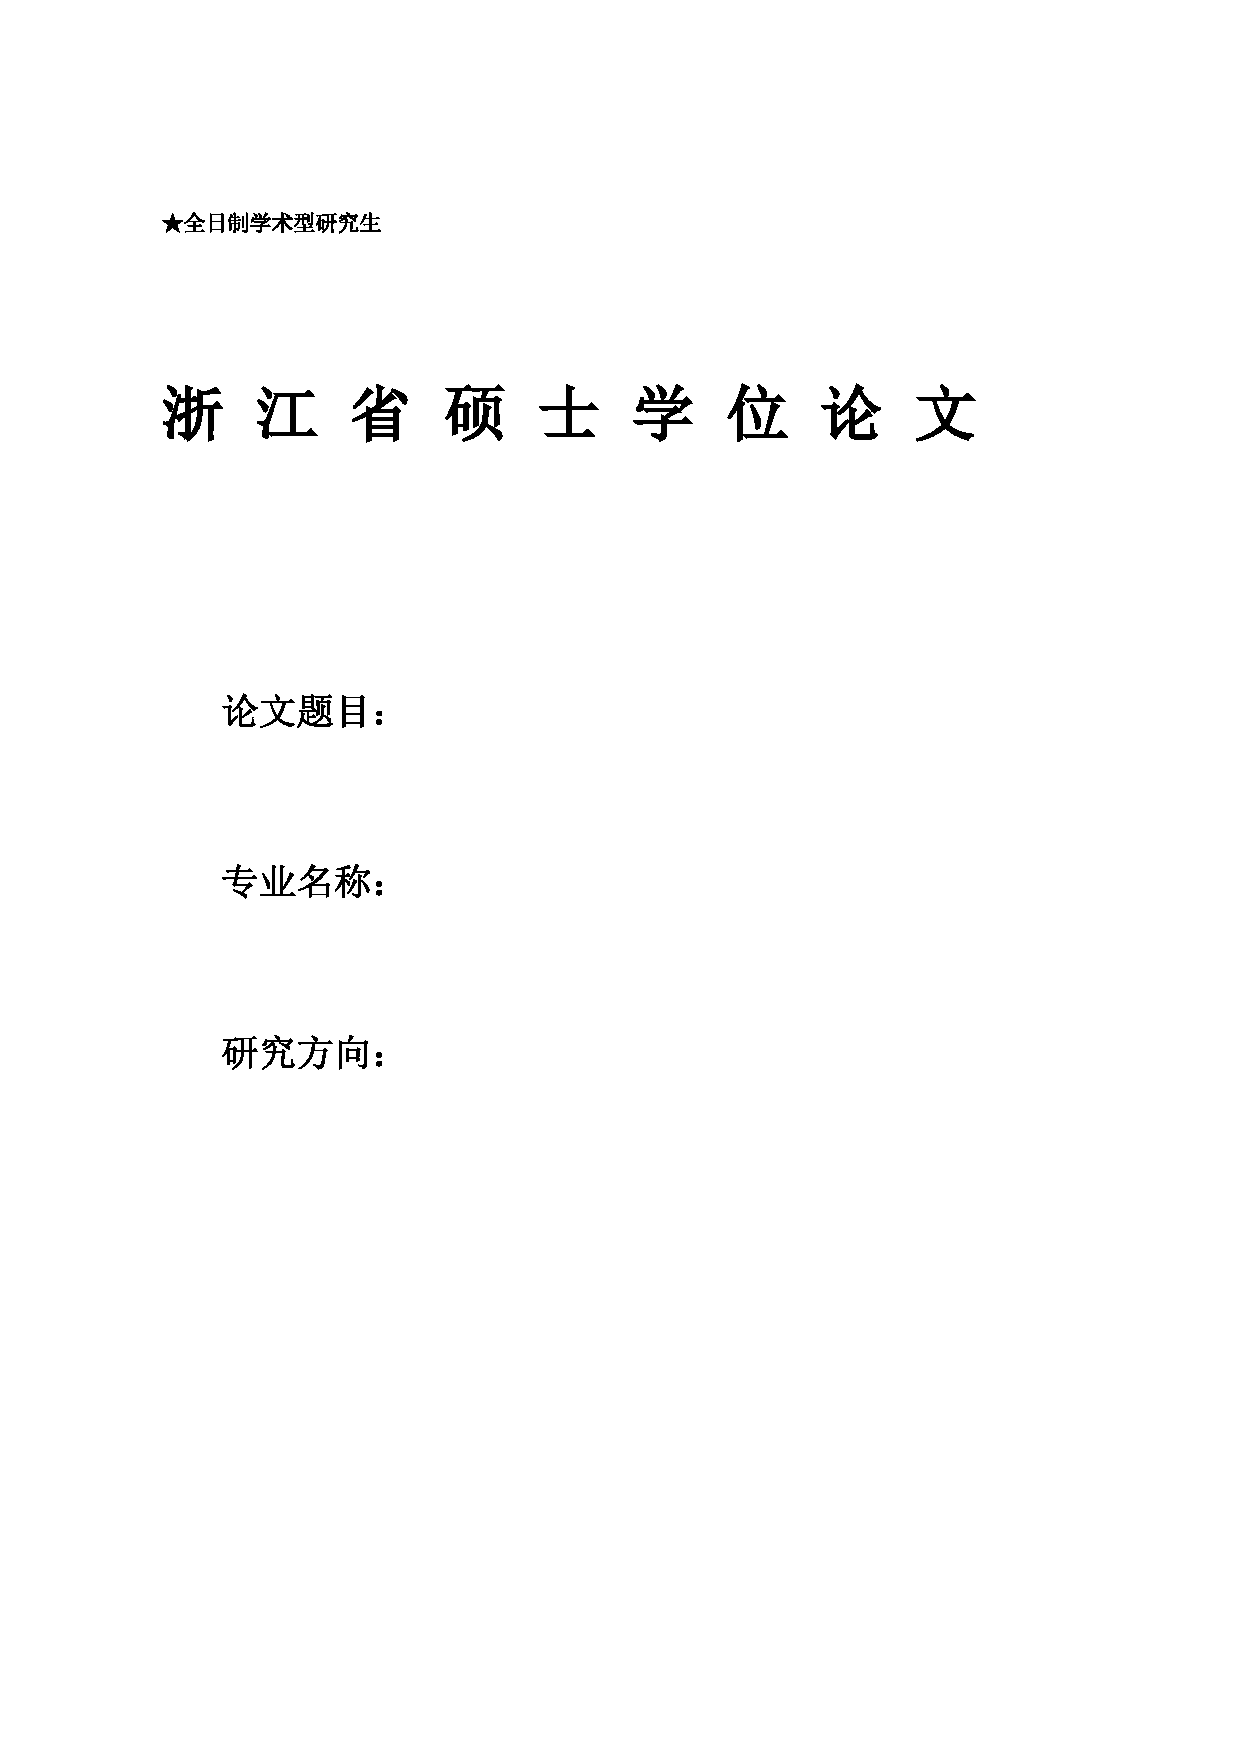
\includepdf[pages={-}]{封面.pdf}

% 插入空白页保持后文奇偶
\cleardoublepage
% 开启页眉、页脚
\pagestyle{HDU-bachelor}

% 页码为罗马数字
\pagenumbering{Roman}

\phantomsection
\addcontentsline{toc}{section}{摘要}
\section*{摘\hspace{2em}要}

随着……。然而,……。此外,……。因此,……。

首先,构建了……。

其次,提出了……。

最后,提出了……。

经过实验验证,……。

\vspace{\baselineskip}\noindent
\textsf{关键词:} 系统,模型

\clearpage
\phantomsection
\addcontentsline{toc}{section}{ABSTRACT}
\section*{\textbf{ABSTRACT}}

Regarding the development of \dots

Firstly, \dots
  
Secondly, \dots
  
Finally, \dots

Through the case studies, \dots

\vspace{\baselineskip}\noindent
\textbf{Key words:} system, model

\clearpage
% 生成目录
\tableofcontents

\clearpage
% 将页码重置为 1
\pagenumbering{arabic}

\section{绪论}

\subsection{研究背景及意义}

示例段落,如图\ref{fig:1}所示。示例引用\cite{levenshtein1966binary}。


\begin{figure}[!ht]
	\centering
	  
\includegraphics[width=0.3\textwidth]{missing}
	  \caption{示例图片}\label{fig:1}
\end{figure}


\floatname{algorithm}{算法}
\renewcommand{\algorithmicrequire}{ \textbf{输入:}}
\renewcommand{\algorithmicensure}{ \textbf{输出:}}
\begin{algorithm}
  \caption{示例算法}\label{alg:1}
  \begin{algorithmic}[1]
    \REQUIRE ~~\\
    $O$,$O'$
    \ENSURE ~~\\
    $set$
    \STATE $set = \{\}$
    \FOR{each $c \in O$ and $c' \in O'$}
    \IF{something is true}
    \STATE do something
    \ENDIF
    \ENDFOR
    \RETURN $set$
  \end{algorithmic}
\end{algorithm}


\clearpage
\section{正文}

\begin{dmath}\label{eq:1}
  Sim(C, C') = {\Sigma_{i=1}^{k_1}\Sigma_{j=1}^{k_1}\sigma(c_i, c_j) \over k_1 + k_2}
\end{dmath}


\begin{lstlisting}[autogobble, language=SPARQL, caption=示例代码, label=code:feature]
    SELECT ?Description
    WHERE {
      ?x rdf:hasDescription ?Description
    }
\end{lstlisting}


\clearpage
% 目录超链接
\phantomsection
% 列出参考文献
\printbibliography[heading=bibintoc]

\clearpage
\phantomsection

\begin{refsection}
  \nocite{self}
  \printbibliography[
    heading=bibintoc,
    title={作者在读期间发表的学术论文及参加的科研项目},
  ]
\end{refsection}

\clearpage
\unnumberedsection{致谢}{致\hspace{2em}谢}

时光荏苒,……。回首岁月,……。

首先我要感谢 ……。

感谢 ……。

感谢 ……。

\end{document}
